\section{HỆ BẤT PHƯƠNG TRÌNH BẬC NHẤT HAI ẨN}

\subsection{TÓM TẮT LÝ THUYẾT}
\subsubsection{Hệ bất phương trình bậc nhất hai ẩn}
\begin{itemize}
	\item [\iconCH] Là hệ bất phương trình gồm hai hay nhiều bất phương trình bậc nhất hai ẩn.
	\item [\iconCH] Cặp số $(x_0;y_0)$ là nghiệm của hệ bất phương trình bậc nhất hai ẩn khi $(x_0;y_0)$ đồng thời là nghiệm của tất cả các bất phương trình trong hệ đó.
\end{itemize}
\subsubsection{Biểu diễn miền nghiệm của hệ bất phương trình bậc nhất hai ẩn}
\begin{itemize}
	\item [\iconCH] Miền nghiệm của hệ là giao các miền nghiệm của các bất phương trình trong hệ.
	\item [\iconCH] Để biểu diễn miền nghiệm của hệ, ta làm như sau:
	\begin{boxdn}
	\begin{itemize}
		\item [$\bullet$] Trên cùng một mặt phẳng tọa độ, xác định miền nghiệm của mỗi bất phương trình bậc nhất hai ẩn trong hệ.
		\item [$\bullet$] Phần giao của các miền nghiệm (phần không bị gạch) là miền nghiệm của hệ bất phương trình đã cho.
	\end{itemize}
	\end{boxdn}
\end{itemize}

\subsection{RÈN LUYỆN KĨ NĂNG GIẢI TOÁN}

\begin{dang}{Biểu diễn miền nghiệm}
\end{dang}
\begin{vd}
	Biểu diễn hình học tập nghiệm của hệ bất phương trình
	$\left\{\begin{aligned}
		x+y &> 1\\
		x-y &<2 \\
	\end{aligned}\right.$.
	\loigiai
	{\immini{
			Vẽ các đường thẳng\\
			$d_1: x+y=1$;\\
			$d_2: x-y=2$.
			
			Vì điểm $M(0,2)$ có tọa độ thỏa mãn các bất phương trình trong hệ nên ta tô đậm các nửa mặt phẳng bờ $d_1,d_2$ không chứa $M$. 
			
			Miền không bị tô đậm trong hình vẽ và không chứa các tia giới hạn miền là miền nghiệm của hệ đã cho.
		}{\begin{tikzpicture}[>=stealth]
				\draw[color=white,fill=black!10] (-2,-2) rectangle (4,3);
				\draw[fill=white,color=white] (-2,3) -- (1.5,-.5) -- (4,2) -- (4,3) -- cycle;
				\draw[->] (0,-2) -- (0,3) node[left]{\scriptsize $y$};
				\draw[->] (-2,0) -- (4,0) node[above]{\scriptsize $x$};
				\draw (0.15,0.1) node[below left]{\scriptsize $O$};
				\draw (-2,3) -- (3,-2) node[right]{\scriptsize $d_1$};
				\draw (0,-2) -- (4,2) node[right]{\scriptsize $d_2$};
				\draw[dashed] (0,-0.5)node[left]{\scriptsize $-\dfrac{1}{2}$} -- (1.5,-.5) node[right]{\scriptsize $I$} -- (1.5,0) node[above]{\scriptsize $\dfrac{3}{2}$};
				\draw (0,2) node[right]{\scriptsize $M$} (0,2) node[left]{\scriptsize $2$} (-0.05,2) -- (0.05,2);
			\end{tikzpicture}
		}
	}
\end{vd} \dongcham{16}
\begin{vd}
	Biểu diễn hình học tập nghiệm của hệ bất phương trình
	$\left\{\begin{aligned}
		x+y &< 2\\
		x-y &>1 \\
		y &>-1
	\end{aligned}\right.$.
	\loigiai
	{\immini{
			Vẽ các đường thẳng\\
			$d_1: x+y=2$,\\
			$d_2: x-y=1$,\\
			$d_3: y=-1$.
			
			Vì điểm $M\biggl(\dfrac{3}{2},0\biggr)$ có tọa độ thỏa mãn các bất phương trình trong hệ nên ta tô đậm các nửa mặt phẳng bờ $d_1,d_2,d_3$ không chứa $M$. Miền không bị tô đậm trong hình vẽ, không bao gồm các đoạn giới hạn miền là miền nghiệm của hệ đã cho.
		}{\begin{tikzpicture}[>=stealth]
				\draw[color=white,fill=black!10] (-2,-2) rectangle (5,3);
				\path (-1,3) coordinate (A1);
				\path (4,-2) coordinate (B1);
				\path (-1,-2) coordinate (A2);
				\path (4,3) coordinate (B2);
				\path (-2,-1) coordinate (A3);
				\path (5,-1) coordinate (B3);
				\path (intersection of A1--B1 and A2--B2) coordinate (A);
				\path (intersection of A1--B1 and A3--B3) coordinate (B);
				\path (intersection of A2--B2 and A3--B3) coordinate (C);
				\draw[fill=white] (A) -- (B) -- (C) -- cycle;
				\draw[->] (0,-2) -- (0,3) node[right]{\scriptsize $y$};
				\draw[->] (-2,0) -- (5,0) node[above]{\scriptsize $x$};
				\draw (0.15,0.1) node[below left]{\scriptsize $O$};
				\draw (A1) -- (B1) node[right]{\scriptsize $d_1$} (A2) -- (B2)node[right]{\scriptsize $d_2$} (A3) -- (B3)node[right]{\scriptsize $d_3$};
				\draw[dashed] (B)node[below]{\scriptsize $B$} -- (B |- 0,0) node[above]{\scriptsize $3$}
				(A-| 0,0)node[left]{\scriptsize $\dfrac{3}{2}$} -- (A)node[above]{\scriptsize $A$} -- (A|- 0,0)node[below]{\scriptsize $\dfrac{3}{2}$};
				\draw (1.5,0)node[above right]{\scriptsize $M$} (C) node[below right]{\scriptsize $C$} (C) node[above left]{\scriptsize $-1$};
			\end{tikzpicture}
		}
	}
\end{vd} \dongcham{10}

\begin{dang}{Tìm giá trị lớn nhất, nhỏ nhất của biểu thức F=ax+by+c trên miền đa giác}
	\begin{listEX}[1]
		\item [\ding{172}] Biểu diễn miền nghiệm (miền đa giác) và tìm tọa độ các đỉnh của đa giác đó.
		\item [\ding{173}] Thay tọa độ các đỉnh của đa giác vào biểu thức $F=ax+by$, chọn GTLN, GTNN.
	\end{listEX}
\end{dang}

\begin{vd}
	Cho hệ bất phương trình $\heva{x + 2y &\le 100 \\ 2x + y &\le 80 \\ x &\ge 0 \\ y &\ge 0}$
	\begin{enumerate}
		\item[a)] Biểu diễn miền nghiệm của hệ bất phương trình.
		\item[b)] Tìm $x, y$ là nghiệm của hệ bất phương trình sao cho $F = 40x + 30y$ đạt giá trị lớn nhất, giá trị nhỏ nhất.
	\end{enumerate}
	\loigiai{
		\begin{enumerate}
			\item[a)] Biểu diễn miền nghiệm:
			\begin{itemize}
				\item Vẽ đường thẳng $d_1\colon x + 2y = 100$, đi qua $(0; 50)$ và $(100; 0)$. Lấy điểm $O(0;0)$, ta thấy $0 + 2 \cdot 0 = 0 \le 100$ (đúng), nên miền nghiệm của bất phương trình $x + 2y \le 100$ là nửa mặt phẳng bờ $d_1$ chứa gốc tọa độ $O$.
				\item Vẽ đường thẳng $d_2\colon 2x + y = 80$, đi qua $(0; 80)$ và $(40; 0)$. Lấy điểm $O(0;0)$, ta thấy $2 \cdot 0 + 0 = 0 \le 80$ (đúng), nên miền nghiệm của bất phương trình $2x + y \le 80$ là nửa mặt phẳng bờ $d_2$ chứa gốc tọa độ $O$.
				\item Miền nghiệm của $x \ge 0$ là nửa mặt phẳng bờ $Oy$ nằm bên phải trục $Oy$.
				\item Miền nghiệm của $y \ge 0$ là nửa mặt phẳng bờ $Ox$ nằm phía trên trục $Ox$.
			\end{itemize}
			
			\begin{center}
				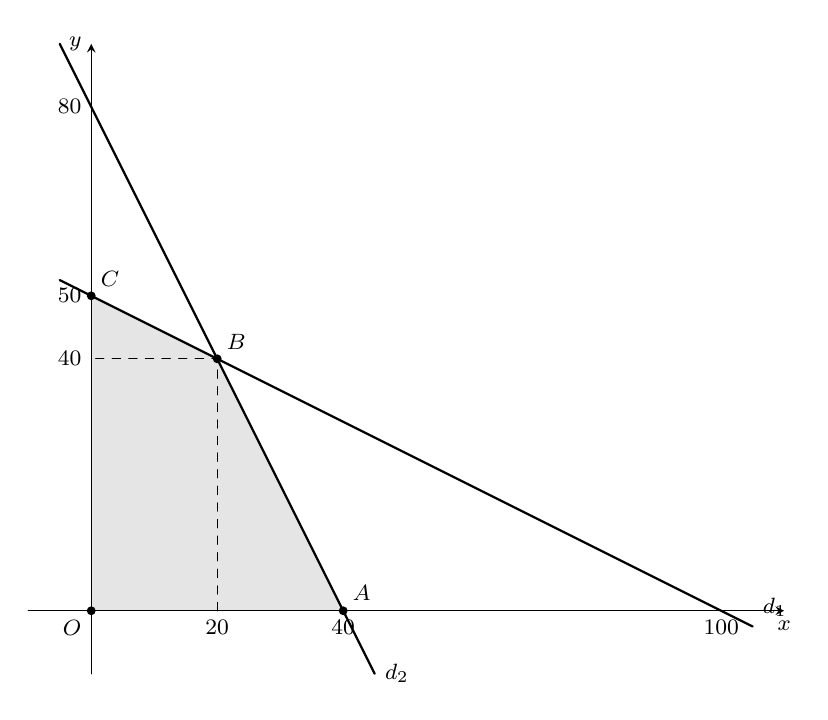
\begin{tikzpicture}[scale=0.08, font=\footnotesize, line join=round, line cap=round, >=stealth]
					% Tô màu miền nghiệm OABC
					\fill[gray!20] (0,0) -- (40,0) -- (20,40) -- (0,50) -- cycle;
					
					% Trục tọa độ
					\draw[->] (-10,0) -- (110,0) node[below] {$x$};
					\draw[->] (0,-10) -- (0,90) node[left] {$y$};
					\node[below left] at (0,0) {$O$};
					
					% Vẽ các đường thẳng
					\draw[thick, domain=-5:105] plot (\x, {-0.5*\x + 50}) node[above right] {$d_1$};
					\draw[thick, domain=-5:45] plot (\x, {-2*\x + 80}) node[right] {$d_2$};
					
					% Gắn nhãn các đỉnh
					\fill (0,0) circle (20pt);
					\fill (40,0) circle (20pt) node[above right] {$A$};
					\fill (20,40) circle (20pt) node[above right] {$B$};
					\fill (0,50) circle (20pt) node[above right] {$C$};
					
					% Các điểm trên trục
					\node[below] at (40,0) {$40$};
					\node[below] at (100,0) {$100$};
					\node[left] at (0,50) {$50$};
					\node[left] at (0,80) {$80$};
					
					% Nét đứt gióng tọa độ điểm B
					\draw[dashed] (20,0) node[below]{$20$} -- (20,40) -- (0,40) node[left]{$40$};
				\end{tikzpicture}
			\end{center}
			
			Giao của các nửa mặt phẳng trên chính là miền nghiệm của hệ bất phương trình. Đó là miền đa giác $OABC$ (kể cả biên) với tọa độ các đỉnh: $O(0;0)$, $A(40;0)$, $B(20;40)$ và $C(0;50)$.
			
			\item[b)] Tìm giá trị lớn nhất, nhỏ nhất của $F = 40x + 30y$ trên miền nghiệm:\\
			Ta tính giá trị của biểu thức $F$ tại các đỉnh của miền đa giác $OABC$:
			\begin{itemize}
				\item Tại đỉnh $O(0;0)$: $F = 40(0) + 30(0) = 0$.
				\item Tại đỉnh $A(40;0)$: $F = 40(40) + 30(0) = 1600$.
				\item Tại đỉnh $B(20;40)$: $F = 40(20) + 30(40) = 800 + 1200 = 2000$.
				\item Tại đỉnh $C(0;50)$: $F = 40(0) + 30(50) = 1500$.
			\end{itemize}
			So sánh các giá trị thu được, ta kết luận:
			\begin{itemize}
				\item Giá trị lớn nhất của $F$ là $2000$, đạt được khi $x = 20, y = 40$.
				\item Giá trị nhỏ nhất của $F$ là $0$, đạt được khi $x = 0, y = 0$.
			\end{itemize}
		\end{enumerate}
	}
\end{vd}
\dongcham{16}
\begin{dang}{Ứng dụng của hệ bất phương trình bậc nhất hai ẩn.}
	Nhiều bài toán trong thực tiễn phải dưa đến việc phải tìm cặp sớ ( $x ; y$ ) thoả mān một hệ bất phương trình bậc nhắt nào đó để một biểu thức dạng $F=a x+$ by dạt dược giá trị lớn nhất hoặc nhỏ nhất. Các bài toán này gọi là các bài toán quy hoạch tuyến tính.
\end{dang}

\begin{vd}
	Một cửa hàng điện tử dự định kinh doanh hai loại ti vi: loại $50$ inch và loại $55$ inch với số vốn ban đầu không vượt quá $1{,}8$ tỉ đồng. Giá nhập và lợi nhuận dự kiến của mỗi loại ti vi được cho trong bảng sau:
	
	\begin{center}
		\begin{tabular}{|l|c|c|}
			\hline
			\diagbox{\textbf{Số tiền}}{\textbf{Loại Tivi}} & \textbf{Ti vi $50$ inch} & \textbf{Ti vi $55$ inch} \\
			\hline
			Giá nhập vào (triệu đồng/$1$ máy) & $15$ & $25$ \\
			\hline
			Lợi nhuận dự kiến (triệu đồng/$1$ máy) & $2$ & $3$ \\
			\hline
		\end{tabular}
	\end{center}
	Cửa hàng ước tính rằng tổng nhu cầu tiêu thụ của thị trường sẽ không vượt quá $100$ chiếc ti vi cả hai loại. Tính số lượng ti vi mỗi loại mà cửa hàng nên nhập về để lợi nhuận thu được (sau khi bán hết hàng nhập về) là lớn nhất.
	
	\loigiai{
		Gọi $x$ và $y$ lần lượt là số lượng ti vi loại $50$ inch và $55$ inch mà cửa hàng dự định nhập về ($x, y \in \mathbb{N}$).
		
		Theo đề bài, ta có các điều kiện ràng buộc sau:
		\begin{itemize}
			\item Tổng nhu cầu tiêu thụ không vượt quá $100$ chiếc nên: $x + y \le 100$.
			\item Đổi $1{,}8$ tỉ đồng $= 1800$ triệu đồng. Tổng số vốn nhập hàng không vượt quá $1800$ triệu đồng nên: 
			$$ 15x + 25y \le 1800 \Leftrightarrow 3x + 5y \le 360. $$
			\item Số lượng tivi không thể âm nên: $x \ge 0$ và $y \ge 0$.
		\end{itemize}
		
		Từ đó, ta có hệ bất phương trình mô tả các điều kiện ràng buộc:
		$$ \begin{cases} x \ge 0 \\ y \ge 0 \\ x + y \le 100 \\ 3x + 5y \le 360 \end{cases} \quad (\mathrm{I}) $$
		
		Lợi nhuận dự kiến thu được là: $F(x, y) = 2x + 3y$ (triệu đồng). 
		Bài toán trở thành tìm giá trị lớn nhất của $F(x, y)$ trên miền nghiệm của hệ bất phương trình $(\mathrm{I})$.
		
		Biểu diễn miền nghiệm của hệ $(\mathrm{I})$ trên mặt phẳng tọa độ $Oxy$:
		\begin{center}
			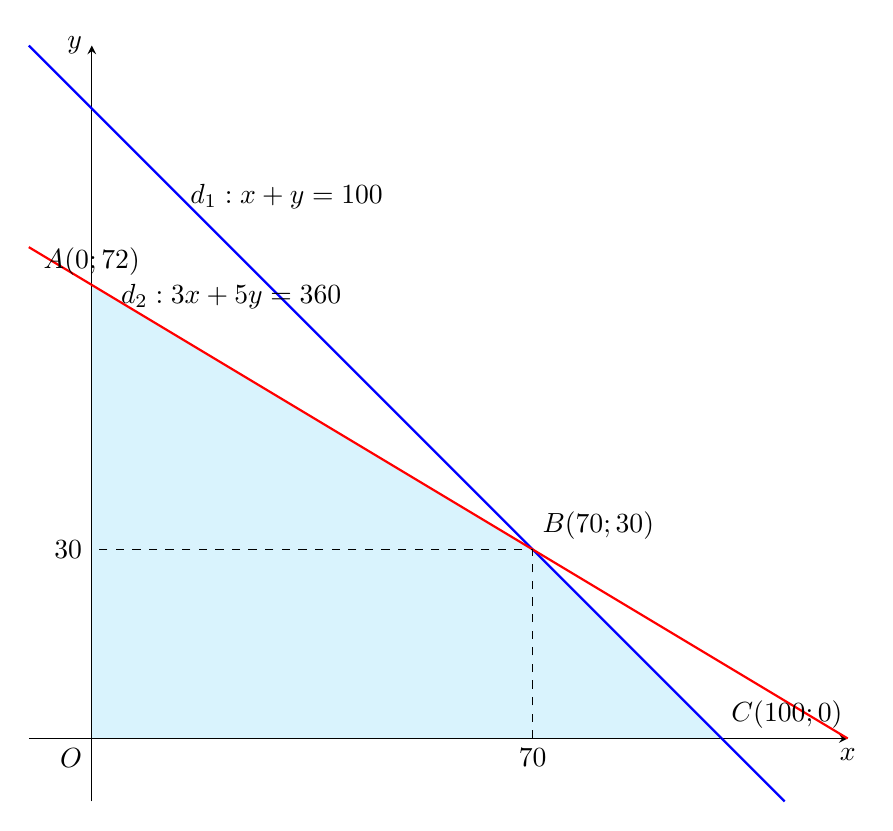
\begin{tikzpicture}[>=stealth, scale=0.08]
				% Tô màu miền nghiệm
				\fill[cyan!15] (0,0) -- (100,0) -- (70,30) -- (0,72) -- cycle;
				
				% Trục tọa độ
				\draw[->] (-10,0) -- (120,0) node[below] {$x$};
				\draw[->] (0,-10) -- (0,110) node[left] {$y$};
				\node[below left] at (0,0) {$O$};
				
				% Vẽ các đường thẳng
				\draw[thick, blue] (-10,110) -- (110,-10) node[pos=0.2, right, black] {$d_1: x+y=100$};
				\draw[thick, red] (-10,78) -- (120,0) node[pos=0.1, right, black] {$d_2: 3x+5y=360$};
				
				% Các đỉnh của đa giác miền nghiệm
				\fill (0,0) circle (1.5pt);
				\fill (100,0) circle (1.5pt) node[above right] {$C(100; 0)$};
				\fill (70,30) circle (1.5pt) node[above right] {$B(70; 30)$};
				\fill (0,72) circle (1.5pt) node[above] {$A(0; 72)$};
				
				% Đường gióng tọa độ điểm B
				\draw[dashed] (70,0) node[below] {$70$} -- (70,30) -- (0,30) node[left] {$30$};
			\end{tikzpicture}
		\end{center}
		
		Miền nghiệm là miền đa giác $OABC$ (kể cả biên) với tọa độ các đỉnh: $O(0; 0)$, $A(0; 72)$, $B(70; 30)$, $C(100; 0)$.
		
		Tính giá trị của biểu thức $F(x, y)$ tại các đỉnh của miền nghiệm:
		\begin{itemize}
			\item Tại $O(0; 0)$: $F(0, 0) = 2 \cdot 0 + 3 \cdot 0 = 0$.
			\item Tại $A(0; 72)$: $F(0, 72) = 2 \cdot 0 + 3 \cdot 72 = 216$.
			\item Tại $B(70; 30)$: $F(70, 30) = 2 \cdot 70 + 3 \cdot 30 = 230$.
			\item Tại $C(100; 0)$: $F(100, 0) = 2 \cdot 100 + 3 \cdot 0 = 200$.
		\end{itemize}
		
		So sánh các giá trị, ta thấy $F(x, y)$ đạt giá trị lớn nhất bằng $230$ khi $x = 70$ và $y = 30$.
		
		\textbf{Kết luận:} Để thu được lợi nhuận lớn nhất, cửa hàng nên nhập về $70$ chiếc ti vi loại $50$ inch và $30$ chiếc ti vi loại $55$ inch.
	}
\end{vd}
\dongcham{10}
\begin{vd} % Câu 3
	(Đề chính thức 2025). Để gây quỹ từ thiện, câu lạc bộ thiện nguyện của một trường THPT tổ chức hoat động bán hàng với hai mặt hàng là nước chanh và khoai chiên. Câu lạc bộ thiết kế hai thực đơn. Thực đơn $1$ có giá $35$ nghìn đồng, bao gồm hai cốc nước chanh và một túi khoai chiên. Thực đơn $2$ có giá $60$ nghìn đồng, bao gồm ba cốc nước chanh và hai túi khoai chiên. Biết rằng câu lạc bộ chỉ làm được không quá $165$ cốc nước chanh và $100$ túi khoai chiên. Số tiền lớn nhất mà câu lạc bộ có thể nhận được sau khi bán hết hàng bằng bao nhiêu nghìn đồng?
%	\shortans[oly]{$3150$}
	\loigiai{
		Ta có:
		\begin{center}
			\begin{tabular}{|c|c|c|c|}
				\hline
				& Cốc nước chanh & Túi khoai chiên & Giá (nghìn đồng) \\ \hline
				Thực đơn $1$: & $2$ & $1$ & $35$ (nghìn đồng) \\ \hline
				$x$ (thực đơn) & $2x$ & $x$ & $35x$(nghìn đồng) \\ \hline
				Thực đơn $2$:  & $3$ & $2$ & $60$(nghìn đồng) \\ \hline
				$y$ (thực đơn)  & $3y$ & $2y$ & $60y$(nghìn đồng) \\ \hline
			\end{tabular}
		\end{center}
		
		Hệ ràng buộc: $\left\{ \begin{gathered}
			x \geqslant 0,\;y \geqslant 0,\;\left( {x,\;y \in \mathbb{Z}} \right) \hfill \\
			2x + 3y \leqslant 165 \hfill \\
			x + 2y \leqslant 100 \hfill \\
		\end{gathered}  \right.$.\\
		Gọi $F\left( {x,\;y} \right)$ (nghìn đồng) là số tiền câu lạc bộ nhận được $ \Rightarrow F\left( {x;\;y} \right) = 35x + 60y$\\
		Tìm GTLN của $F\left( {x;\;y} \right)$ thỏa mãn $\left\{ \begin{gathered}
			x \geqslant 0,\;y \geqslant 0,\;\left( {x,\;y \in \mathbb{Z}} \right) \hfill \\
			2x + 3y \leqslant 165 \hfill \\
			x + 2y \leqslant 100 \hfill \\
		\end{gathered}  \right.$
		\begin{center}
			\begin{tikzpicture}[scale=0.8, font=\footnotesize,line join=round, line cap=round, >=stealth]
				\coordinate (O) at (0,0);
				\coordinate (x) at (11,0);
				\coordinate (y) at (0,8);
				\coordinate (A) at (0,5);
				\coordinate (B) at (3,3.5);
				\coordinate (C) at (8.25,0);
				\draw[->]($(O)!-0.2!(x)$)--(x);
				\draw[->]($(O)!-0.2!(y)$)--(y);
				\draw[thin]($(A)!-0.5!(B)$)--($(A)!3.5!(B)$);
				\draw[thin]($(B)!-1!(C)$)--($(B)!1.1!(C)$);
				\fill[pattern=north east lines](O)--(A)--(B)--(C)--cycle;
				\foreach \i/\g in {O/120,x/-90,y/45,A/135,B/10,C/-90}{\draw[fill=black](\i) circle (1pt) ($(\i)+(\g:4mm)$) node[scale=1]{$\i$};}
				\draw ($(B)!-1!(C)$) node[above]{$2x+3y=165$};
				\draw ($(A)!-0.5!(B)$) node[below left]{$x+2y=100$};
			\end{tikzpicture}
		\end{center}
		Miền nghiệm của hệ bất phương trình là miền tứ giác $OABC$ (kể cả biên). Tọa độ của các đỉnh tứ giác đó là $O(0;0)$, $A(0;50)$, $B(30;35)$, $C(82,5;0)$. Thế lần lượt tọa độ các đỉnh của tứ giác vào hàm $F = 35x + 60y$, ta được:\\
		Tại $O(0;0)$:$F = 35.0 + 60.0 = 0;$\\
		Tại $A(0;50)$: $F = 35.0 + 60.50 = 3000;$\\
		Tại $B(30;35)$: $F = 35.30 + 60.35 = 3150;$\\
		Tại $C(82,5;0)$: $F = 35.82,5 + 60.0 = 2887,5;$\\
		Ta thấy $F\left( {x;\;y} \right) = 35x + 60y$ đạt giá trị lớn nhất bằng $3150$ nghìn đồng tại điểm $B(30;35)$.\\Vậy số tiền lớn nhất mà câu lạc bộ có thể nhận được sau khi bán hết hàng bằng $3150$ nghìn đồng.}
\end{vd}
\dongcham{10}

\begin{vd}%[BG10-2022]%[Toanvo]%[0D4G4-4]
	Một gia đình cần ít nhất $900$ đơn vị protein và $400$ đơn vị lipit trong thức ăn mỗi ngày. Mỗi kg thịt bò chứa $800$ đơn vị protein và $200$ đơn vị lipit. Mỗi kg thịt lợn chứa $600$ đơn vị protein và $400$ đơn vị lipit. Biết rằng mỗi ngày gia đình này chỉ mua tối đa $1{,}5$ kg thịt bò và $1$ kg thịt lợn, giá tiền $1$ kg thịt bò là $200$ nghìn đồng, $1$ kg thịt lợn là $100$ nghìn đồng. Hỏi gia đình đó phải mua bao nhiêu kg thịt mỗi loại để số tiền bỏ ra là ít nhất.
	\loigiai{
		Gọi số kg thịt bò cần mua là $x$ (kg); số kg thịt lợn cần mua là $y$ (kg). Điều kiện: $0 \leq x \leq 1{,}5, 0 \leq y \leq 1$.\\
		Khi đó số đơn vị protein là $800x+600y$.\\
		Số đơn vị lipit là $200x+400y$.\\
		Ta có hệ bất phương trình $$\heva{&0\leq x\leq 1{,}5\\&0\leq y\leq 1\\&800x+600y\geq 900\\&200x+400y\geq200}\Leftrightarrow\heva{&0\leq x\leq 1{,}5\\&0\leq y\leq 1\\&8x+6y\geq9\\&x+2y\geq2.}$$	
		Vẽ các đường thẳng $(d_1)\colon x=1{,}5$, $(d_2)\colon y=1$, $(d_3)\colon 8x+6y=9$, $(d_4)\colon x+2y=2$. Ta được miền nghiệm của hệ bất phương trình là phần tô đậm trong hình vẽ.
		\begin{center}
			\begin{tikzpicture}[line join = round, line cap = round, >=stealth, font=\footnotesize, scale=1.2]
				\tikzset{label style/.style={font=\footnotesize}}
				\def \xmin{-3.5}
				\def \xmax{5.5}
				\def \ymin{-1.5}
				\def \ymax{6}
				\tkzDefPoints{0.375/1/A, 1.5/1/B, 1.5/0.25/C, 0.6/0.7/D}
				\draw[gray!20](\xmin,\ymin) grid (\xmax,\ymax);
				\draw [->](\xmin,0)--(0,0)node[below left]{$O$}--(\xmax,0)node[above]{$x$};
				\draw [->](0,\ymin)--(0,\ymax)node[right]{$y$};
				\foreach \x in {-3,-2,-1,1,2,3,4,5} \draw[shift={(\x,0)}] (0pt,2pt)--(0pt,-2pt) node[below]{$\x$};
				\foreach \y in {-1,2,3,4,5} \draw [shift={(0,\y)}] (2pt,0pt)--(-2pt,0pt) node[left]{$\y$};
				\draw [shift={(0,1)}] (2pt,0pt)--(-2pt,0pt) node[below left]{$1$};
				\tkzDrawLine[add=6 and 2](B,C)
				%\tkzDrawLine[add=0.5 and 0.5](B,C A,B A,D D,C)
				\tkzDrawLine[add=3 and 3](A,B)
				\tkzDrawLine[add=12 and 6](A,D)
				\tkzDrawLines[add=4 and 2](D,C)
				\tkzDrawPoints[fill=black](A,B,C,D)
				\tkzLabelPoints[above right](A,B,C)
				\tkzLabelPoints[below](D)
				\tkzFillPolygon[color=cyan,fill opacity=.5](A,B,C,D)
				\tkzLabelLine[pos=7,right](C,B){$(d_1)$}
				\tkzLabelLine[pos=3.5,above right](A,B){$(d_2)$}
				\tkzLabelLine[pos=12,above right](D,A){$(d_3)$}
				\tkzLabelLine[pos=5,above right](C,D){$(d_4)$}
			\end{tikzpicture}
		\end{center}
		Ta có 
		{\allowdisplaybreaks
			\begin{eqnarray*}
				&&A\left(\dfrac{3}{8};1\right)=(d_3) \cap (d_2), B(1{,}5;1)=(d_1) \cap (d_2),\\
				&&C(1{,}5;0{,}25)=(d_1) \cap (d_4), D\left(\dfrac{3}{5};\dfrac{7}{10}\right)=(d_3) \cap (d_4).
			\end{eqnarray*}
		}
		Số tiền bỏ ra là $f(x,y)=200x+100y$ (nghìn đồng).
		\begin{center}
			\renewcommand\arraystretch{1.6}
			\renewcommand{\tabcolsep}{6mm}
			\begin{tabular}{|c|c|c|c|c|}
				\hline 
				$M(x;y)$& $A$ & $B$ & $C$ & $D$ \\ 
				\hline 
				$f(x,y)=200x+100y$& $175$ & $400$ & $325$ & $190$ \\ 
				\hline 
			\end{tabular} 
		\end{center}
		Do đó $f(x,y)$ đạt giá trị nhỏ nhất tại $A\left(\dfrac{3}{8};1\right)$.\\
		Vậy để số tiền bỏ ra nhỏ nhất thì cần mua $\dfrac{3}{8}$ kg thịt bò và $1$ kg thịt lợn.
	}
\end{vd}
\dongcham{14}

\begin{vd}
	Trong một cuộc thi pha chế, mỗi đội chơi được sử dụng tối đa $ 24 g $ hương liệu, $ 9 $ lít nước và $ 210 g $ đường để pha chế nước cam và nước táo. Để pha chế $ 1 $ lít nước cam cần $ 30 g $ đường, $ 1 $ lít nước và $ 1 g $ hương liệu; pha chế $ 1 $ lít nước táo cần $ 10 g $ đường, $ 1 $ lít nước và $ 4 g $ hương liệu. Mỗi lít nước cam nhận được $ 60 $ điểm thưởng, mỗi lít nước táo nhận được $ 80 $ điển thưởng.
	Hỏi cần pha chế bao nhiêu lít nước trái cây mỗi loại để được số điểm thưởng là lớn nhất.
	\loigiai{
		\begin{itemize}
			\item Gọi $ x, y $ lần lượt là số lít nước cam và táo của một đội pha chế $ (x, y\ge 0). $
			\item Số điểm thưởng của đội chơi này là $ f(x;y)=60x+80y. $
			\item Số gam đường cần dùng là $ 30x+10y. $
			\item Số lít nước cần dùng là $ x+y. $
			\item Số gam hương liệu cần dùng là $ x+4y $
			\item Vì trong cuộc thi pha chế, mỗi đội chơi sử dụng tối đa $ 24 g $ hương liệu, $ 9 $ lít nước và $ 210 g $ đường nên ta có hệ bất phương trình $ \heva{&30x+10y\le 210\\&x+y\le 9\\ &x+4y\le 24\\&x, y\ge 0}\Leftrightarrow   \heva{&3x+y\le 21\\&x+y\le 9\\ &x+4y\le 24\\&x, y\ge 0} (*).$
			\item Bài toán trở thành tìm giá trị lớn nhất của hàm số $ f(x;y) $ trên miền nghiệm của hệ bất phương
			trình $ (*). $
			\item Miền nghiệm của hệ bất phương trình$  (*) $ là ngũ giác $ OABCD $ (kể cả biên).
			Hàm số $ f(x;y)=60x+80y $ sẽ đạt giá trị lớn nhất trên miền nghiệm của hệ bất phương trình $ (*) $ khi $ (x;y) $ là toạ độ của một trong các đỉnh $ O(0;0), A(7;0), B(6;3), C(4;5), D(0;6). $
			\item Ta có: $ f(0;0)=0; f(7;0)=420; f(6;3)=600; f(4;5)=640; f(0;6)=480. $\\
			Suy ra $ f(4;5) $ là giá trị lớn nhất của hàm số $ f(x;y) $ trên miền nghiệm của hệ $ (*).  $\\
			Như vậy để được số điểm thưởng là lớn nhất cần pha chế $ 6 $ lít nước cam và $ 5 $ lít nước táo.
			
		\end{itemize}
		\begin{center}
			\begin{tikzpicture}[line width=1pt,>=stealth,x=1cm,y=1cm,scale=0.6]
				\draw[->] (-1,0)--(10.3,0)
				node[below]{\footnotesize $ x $};
				\draw[->] (0,-1)--(0,10.3)
				node[right]{\footnotesize $ y $};
				\draw (0,0) node[below left]{\footnotesize $ O$};
				\clip (-1,-1) rectangle (10,10);
				\draw[smooth,domain=-5:24] plot (\x,{-3*\x+21});
				\draw[smooth,domain=-5:24] plot (\x,{-\x+9});
				\draw[smooth,domain=-5:24] plot (\x,{-0.25*\x+6});
				\fill[pattern=north west lines]
				(-1,-1)--(-1,22)--(0,22)--(0,-1)--cycle;
				\fill[pattern=north west lines]
				(-1,-1)--(-1,0)--(25,0)--(25,-1)--cycle;
				\fill[pattern=north west lines]
				(-0.3,22)--(7.3,-1)--(25,-1)--(25,22)--cycle;
				\fill[pattern=north west lines]
				(0,6)--(0,21)--(5.5,4.7)--cycle;
				\fill[pattern=north west lines]
				(6,3)--(0,8)--(0,21)--cycle;
				\draw (7,0) node[above left]{\footnotesize$A$};
				\draw (7,0) node[below]{\footnotesize$7$};
				\draw (6,3) node[right]{\footnotesize$B$};
				\draw[dashed] (0,3)--(6,3);
				\draw (0,3) node[left]{\footnotesize$3$};
				\draw[dashed] (6,0)--(6,3);
				\draw (6,0) node[below]{\footnotesize$6$};
				\draw (4,5) node[below left]{\footnotesize$C$};
				\draw[dashed] (0,5)--(4,5);
				\draw (0,5) node[left]{\footnotesize$5$};
				\draw[dashed] (4,0)--(4,5);
				\draw (4,0) node[below]{\footnotesize$4$};
				\draw (0,6) node[below right]{\footnotesize$D$};
				\draw (0,6) node[above right]{\footnotesize$6$};
			\end{tikzpicture}
		\end{center}
	}
\end{vd} \dongcham{18}


\begin{vd}
	Cô Hạnh đầu tư không quá $1{,}2$ tỉ đồng vào hai loại cổ phiếu: cổ phiếu $A$ dự kiến chi trả cổ tức bằng tiền với tỉ lệ $4\%$; cổ phiếu $B$ rủi ro cao dự kiến chi trả cổ tức bằng tiền với tỉ lệ $10\%$. Giá cổ phiếu $A$ là $15\,000$ đồng/$1$ cổ phiếu, giá cổ phiếu $B$ là $25\,000$ đồng/$1$ cổ phiếu. Để giảm thiểu rủi ro, cô Hạnh quyết định mua số lượng cổ phiếu $B$ không quá $12\,000$ cổ phiếu. Hỏi cô Hạnh nên đầu tư mỗi loại bao nhiêu cổ phiếu để lợi nhuận thu được là lớn nhất?
	\loigiai{
		Đổi $1{,}2$ tỉ đồng $= 1\,200\,000\,000$ đồng.
		
		Gọi $x$ và $y$ lần lượt là số lượng cổ phiếu $A$ và cổ phiếu $B$ mà cô Hạnh dự định đầu tư ($x \ge 0, y \ge 0$ và $x, y \in \mathbb{N}$).
		
		Theo đề bài, ta có các điều kiện ràng buộc sau:
		\begin{itemize}
			\item Tổng số tiền đầu tư không vượt quá $1{,}2$ tỉ đồng nên: 
			$$ 15\,000x + 25\,000y \le 1\,200\,000\,000 \Leftrightarrow 3x + 5y \le 240\,000. $$
			\item Số lượng cổ phiếu $B$ không quá $12\,000$ nên: $y \le 12\,000$.
		\end{itemize}
		
		Ta có hệ bất phương trình mô tả các điều kiện ràng buộc:
		$$ \begin{cases} x \ge 0 \\ y \ge 0 \\ y \le 12\,000 \\ 3x + 5y \le 240\,000 \end{cases} \quad (\mathrm{I}) $$
		
		Lợi nhuận thu được từ $1$ cổ phiếu $A$ là: $15\,000 \cdot 4\% = 600$ (đồng).\\
		Lợi nhuận thu được từ $1$ cổ phiếu $B$ là: $25\,000 \cdot 10\% = 2\,500$ (đồng).\\
		Tổng lợi nhuận dự kiến thu được là: $F(x, y) = 600x + 2\,500y$ (đồng).
		
		Bài toán trở thành tìm giá trị lớn nhất của biểu thức $F(x, y)$ trên miền nghiệm của hệ bất phương trình $(\mathrm{I})$.
		
		Biểu diễn miền nghiệm của hệ $(\mathrm{I})$ trên mặt phẳng tọa độ $Oxy$:
		\begin{center}
			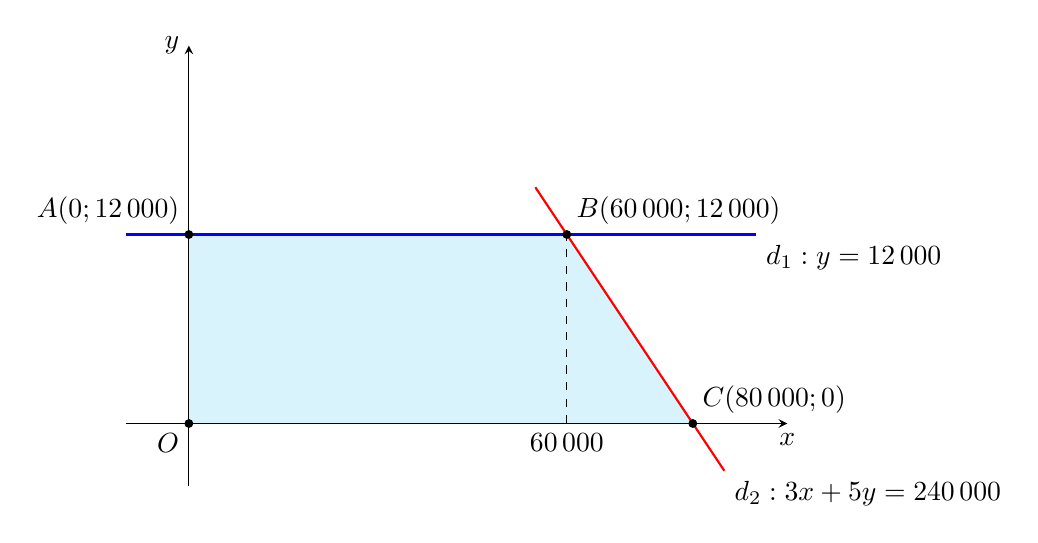
\begin{tikzpicture}[>=stealth, scale=0.8]
				% Tô màu miền nghiệm
				\fill[cyan!15] (0,0) -- (8,0) -- (6,3) -- (0,3) -- cycle;
				
				% Trục tọa độ
				\draw[->] (-1,0) -- (9.5,0) node[below] {$x$};
				\draw[->] (0,-1) -- (0,6) node[left] {$y$};
				\node[below left] at (0,0) {$O$};
				
				% Vẽ các đường thẳng
				\draw[thick, blue] (-1, 3) -- (9, 3) node[below right, black] {$d_1: y = 12\,000$};
				\draw[domain=5.5:8.5, thick, red] plot (\x, {-1.5*\x + 12}) node[below right, black] {$d_2: 3x+5y=240\,000$};
				
				% Các đỉnh của đa giác miền nghiệm
				\fill (0,0) circle (2pt);
				\fill (8,0) circle (2pt) node[above right] {$C(80\,000; 0)$};
				\fill (6,3) circle (2pt) node[above right] {$B(60\,000; 12\,000)$};
				\fill (0,3) circle (2pt) node[above left] {$A(0; 12\,000)$};
				
				% Đường gióng
				\draw[dashed] (6,0) node[below] {$60\,000$} -- (6,3);
			\end{tikzpicture}
		\end{center}
		\textit{(Lưu ý: Tỉ lệ trên các trục tọa độ trong hình vẽ mang tính chất minh họa để xác định đúng hình dáng đa giác miền nghiệm).}
		
		Miền nghiệm là miền tứ giác $OABC$ (kể cả biên) với tọa độ các đỉnh: $O(0; 0)$, $A(0; 12\,000)$, $B(60\,000; 12\,000)$, $C(80\,000; 0)$.
		
		Tính giá trị của biểu thức $F(x, y)$ tại các đỉnh của miền nghiệm:
		\begin{itemize}
			\item Tại $O(0; 0)$: $F(0, 0) = 0$.
			\item Tại $A(0; 12\,000)$: $F(0; 12\,000) = 600 \cdot 0 + 2\,500 \cdot 12\,000 = 30\,000\,000$.
			\item Tại $B(60\,000; 12\,000)$: $F(60\,000; 12\,000) = 600 \cdot 60\,000 + 2\,500 \cdot 12\,000 = 66\,000\,000$.
			\item Tại $C(80\,000; 0)$: $F(80\,000; 0) = 600 \cdot 80\,000 + 2\,500 \cdot 0 = 48\,000\,000$.
		\end{itemize}
		
		So sánh các giá trị, ta thấy $F(x, y)$ đạt giá trị lớn nhất bằng $66\,000\,000$ (đồng) khi $x = 60\,000$ và $y = 12\,000$.
		
		\textbf{Kết luận:} Để thu được lợi nhuận lớn nhất, cô Hạnh nên đầu tư mua $60\,000$ cổ phiếu $A$ và $12\,000$ cổ phiếu $B$.
	}
\end{vd}
\dongcham{20}
\boxmini{BÀI TẬP TỔNG HỢP TỰ LUYỆN}

\begin{baitap}%[Lâm Hữu Phước]%[0D4B4]
	Biểu diễn hình học tập nghiệm của hệ bất phương trình
	$\left\{\begin{aligned}
		x+2y &\geq 1\\
		3x-y & \leq 2 \\
	\end{aligned}\right.$.
\end{baitap} \cham{9}

\begin{baitap}
	Biểu diễn hình học tập nghiệm của hệ bất phương trình
	$\left\{\begin{aligned}
		2x+y &\geq 2\\
		x-2y &\leq 1 \\
		y &\leq 2\\
		x &\leq 3
	\end{aligned}\right.$.
	\loigiai
	{\immini{
			Vẽ các đường thẳng\\
			$d_1: 2x+y=2$,\\
			$d_2: x-2y=1$,\\
			$d_3: y=2$,
			$d_4: x=3$.
			
			Vì điểm $M(2,1)$ có tọa độ thỏa mãn các bất phương trình trong hệ nên ta tô đậm các nửa mặt phẳng bờ $d_1,d_2,d_3,d_4$ không chứa $M$. Miền không bị tô đậm trong hình vẽ là miền nghiệm của hệ đã cho bao gồm các đoạn thẳng xác định miền.
		}{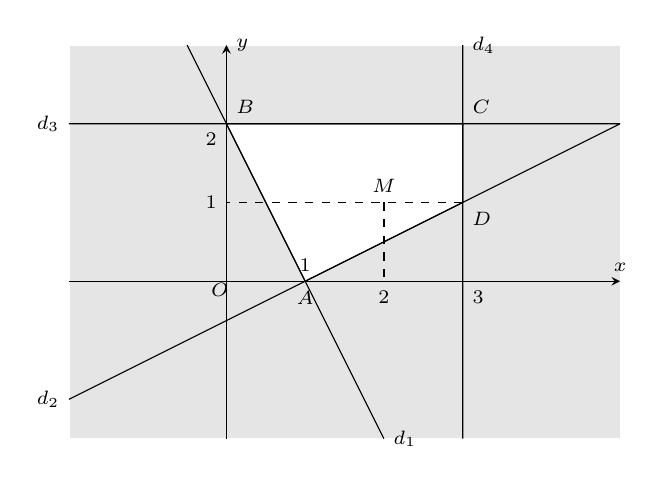
\begin{tikzpicture}[>=stealth]
				\draw[color=white,fill=black!10] (-2,-2) rectangle (5,3);
				\path (-1/2,3) coordinate (A1);
				\path (2,-2) coordinate (B1);
				\path (-2,-3/2) coordinate (A2);
				\path (5,2) coordinate (B2);
				\path (-2,2) coordinate (A3);
				\path (5,2) coordinate (B3);
				\path (3,-2) coordinate (A4);
				\path (3,3) coordinate (B4);
				\path (intersection of A1--B1 and A2--B2) coordinate (A);
				\path (intersection of A1--B1 and A3--B3) coordinate (B);
				\path (intersection of A3--B3 and A4--B4) coordinate (C);
				\path (intersection of A2--B2 and A4--B4) coordinate (D);
				\draw[fill=white] (A) -- (B) -- (C) -- (D) -- cycle;
				\draw[->] (0,-2) -- (0,3) node[right]{\scriptsize $y$};
				\draw[->] (-2,0) -- (5,0) node[above]{\scriptsize $x$};
				\draw (0.15,0.1) node[below left]{\scriptsize $O$};
				\draw (A1) -- (B1) node[right]{\scriptsize $d_1$} (A2)node[left]{\scriptsize $d_2$} -- (B2) (A3)node[left]{\scriptsize $d_3$} -- (B3) (A4) -- (B4) node[right]{\scriptsize $d_4$};
				\draw[dashed] (A) node[above]{\scriptsize $1$} (A) node[below]{\scriptsize $A$} (B) node[below left]{\scriptsize $2$} (B) node[above right]{\scriptsize $B$} (C) node[above right]{\scriptsize $C$} (C|- 0,0) node[below right]{\scriptsize $3$} (D) node[below right]{\scriptsize $D$} -- (D-| 0,0) node[left]{\scriptsize $1$} (2,1) node[above]{\scriptsize $M$} -- (2,0)node[below]{\scriptsize $2$};
			\end{tikzpicture}
		}
	}
\end{baitap} \cham{10}

\begin{baitap}%Câu 3.4
	(Đề thi chính thức 2025). Để gây quỹ từ thiện, câu lạc bộ thiện nguyện của một trường THPT tổ chức hoạt động bán hàng với hai mặt hàng là nước chanh và khoai chiên. Câu lạc bộ thiết kế hai thực đơn. Thực đơn 1 có giá $30$ nghìn đồng, bao gồm hai cốc nước chanh và một túi khoai chiên. Thực đơn $2$ có giá $50$ nghìn đồng, bao gồm ba cốc nước chanh và hai túi khoai chiên. Biết rằng câu lạc bộ chỉ làm được không quá $165$ cốc nước chanh và $100$ túi khoai chiên. Số tiền lớn nhất mà câu lạc bộ có thể nhận được sau khi bán hết hàng bằng bao nhiêu nghìn đồng?
%	\shortans{$2650$}
\end{baitap}

\begin{baitap}
	Một hộ nông dân định trồng đậu và cà trên diện tích $8$ ha. Nếu trồng đậu thì cần $20$ công và thu $3000000$ đồng trên diện tích mỗi ha, nếu trồng cà thì cần $30$ công và thu $4000000$ đồng trên diện tích mỗi ha. Hỏi cần trồng mỗi loại cây trên với diện tích là bao nhiêu để thu được nhiều tiền nhất biết rằng tổng số công không quá $180$?
	\loigiai{
		Gọi số ha đậu và cà mà hộ nông dân này trồng lần lượt là $x$ và $y (x,y\ge 0).$\\
		Lợi nhuận thu được là $f(x;y)=3000000x+4000000y$ (đồng).\\
		Tổng số công dùng để trông $x$ ha đậu và $y$ ha cà là $20x+30y.$\\
		Ta có hệ bất phương trình sau $\heva{&x+y\le 8\\&20x+30y\le 180\\&x, y\ge 0}\Leftrightarrow \heva{&x+y\le 8\\&2x+3y\le 18\\&x, y\ge 0}.$\\
		Bài toán trở thành tìm giá trị lớn nhất của hàm số $f(x;y)$ trên miền nghiệm của hệ bất phương trình $(*)$. Miền nghiệm của hệ bất phương trình $(*)$ là tứ giác $OABC$ (kể cả biên).\\
		Hàm số $f(x;y)$ sẽ đạt giá trị lớn nhất khi $(x;y)$ là tọa độ của một trong các đỉnh $O(0;0)$,  $ A(8;0)$,  $ B(6;2)$,  $ C(0;6)$.\\
		Ta có: $f(0;0)=0, f(8;0)=24000000, f(6;2)=26000000, f(0;6)=2400000.$\\
		Suy ra $f(x;y)$ lớn nhất khi $(x;y)=(6;2)$ tức là hộ nông dân này cần phải tròng $6$ ha đậu và $2$ ha cà thì sẽ thu về lợi nhuận lớn nhất. 
		\begin{center}
			\begin{tikzpicture}[line width=1pt,>=stealth,x=1cm,y=1cm,scale=0.5]
				\draw[->] (-1,0)--(10.2,0)
				node[below]{\footnotesize $ x $};
				\draw[->] (0,-1)--(0,10.2)
				node[right]{\footnotesize $ y $};
				\draw (0,0) node[below left]{\footnotesize $O$};
				\clip (-1,-1) rectangle (10,10);
				\draw[smooth,domain=-1:10] plot (\x,{-\x+8});
				\draw[smooth,domain=-1:10] plot (\x,{-0.67*\x+6});
				%\draw[-] (4,-1) -- (4,10);
				\fill[pattern=north west lines]
				(-6,10)--(10,10)--(10,-0.6)--cycle;
				\fill[pattern=north west lines]
				(-1,0)--(10,0)--(10,-1)--(-1,-1)--cycle;
				\fill[pattern=north west lines]
				(-1,-1)--(-1,10)--(0,10)--(0,-1)--cycle;
				\fill[pattern=north west lines]
				(-2,10)--(10,10)--(10,-2)--cycle;
				\draw (8,0) node[above]{\footnotesize$A$};
				\draw (8,0) node[below left]{\footnotesize$8$};
				\draw (6,2) node[right]{\footnotesize$B$};
				\draw (6,0) node[below]{\footnotesize$6$};
				\draw[dashed] (0,2)--(6,2);
				\draw (0,2) node[left]{\footnotesize$2$};
				\draw[dashed] (6,0)--(6,2);
				\draw (0,6) node[right]{\footnotesize $C$};
				\draw (0,6) node[left]{\footnotesize $6$};
			\end{tikzpicture}
		\end{center}
	}
\end{baitap} \cham{17}

\begin{baitap}%[0D4K4-3]%Câu 23
	Một xưởng sản xuất có $ 2 $ máy đặc chủng $A$ và $B$ để sản xuất $ 2 $ loại sản phẩm $X$ và $Y$. Để sản xuất $ 1 $ tấn sản phẩm loại $X$ cần dùng máy $A $ trong $ 6 $ giờ và dùng máy $ B$ trong $ 2 $ giờ. Để sản xuất $ 1 $ tấn sản phẩm loại $Y  $ cần dùng máy $ A $ trong $ 2 $ giờ và dùng máy $B$ trong $ 2 $ giờ. Cho biết mỗi máy không thể sản xuất đồng thời $ 2 $ loại sản phẩm. Máy $A$ làm việc không quá $ 12 $ giờ $ 1 $ ngày, máy $B$ làm việc không quá $ 8 $ giờ $ 1 $ ngày. Một tấn sản phẩm loại $X$ lãi $ 10 $ triệu đồng và $ 1 $ tấn sản phẩm loại $Y$ lãi $ 8 $ triệu đồng. Hãy lập kế hoạch sản xuất mỗi ngày sao cho tiền lãi thu được là lớn nhất.
	\dapso{$ 1 $ tấn sản phẩm loại $ X $ và $ 3 $ tấn sản phẩm loại $ Y $.}
	\loigiai{
		\immini{	Gọi $x$, $y$ là số tấn sản phẩm loại $X$, $Y$ cần sản xuất ($ x,y\ge 0 $).\\
			Theo giả thiết bài toán ta có $ \heva{&x\ge 0\\&y\ge 0\\&3x+y\le 6\\&x+y\le 4.} $\\
			Số tiền lãi thu về là $ F(x;y) =10x+8y $ (triệu đồng).\\
			Biểu diễn miền nghiệm của hệ bất phương trình như hình bên.}{\begin{tikzpicture}[line join=round, line cap=round,>=stealth,thick]
				\tikzset{every node/.style={scale=0.9}}
				\begin{scope}
					\clip (-1,-1) rectangle (6,6);
					\fill[pattern=north east lines] (0,-1)--(-1,-1)--(-1,6)--(0,6)--cycle;
					\fill[pattern=north east lines] (-1,0)--(-1,-1)--(6,-1)--(6,0)--cycle;
					\fill[pattern=north east lines] (-2,12)--(7,12)--(7,-15)--cycle;
					\fill[pattern=north east lines] (-3,7)--(7,7)--(7,-3)--cycle;
					\draw (0,6)--(2.33,-1) node [pos=0.45, above, sloped] {};
					\draw (-2,6)--(5,-1) node [pos=0.45, above, sloped] {};
				\end{scope}
				
				\draw[->] (-1,0)--(6,0) node[below]{$x$};
				\draw[->] (0,-1)--(0,6) node[left]{$y$};
				\draw (0,0) node[below left]{$O$};
				\draw[fill=black] (2,0) circle (1pt) node[below left]{$ C $};
				\draw[fill=black] (0,4) circle (1pt) node[shift={(-150:0.3)}]{$ A $};
				\draw[fill=black] (1,3) circle (1pt) node[shift={(80:0.3 )}]{$ B $};
				\draw[fill=black] (2,0) circle (1pt) node[shift={(60:0.3 )}]{$ 2 $};
				\draw[fill=black] (0,4) circle (1pt) node[shift={(20:0.3)}]{$ 4 $};
				%		\draw[fill=black] (1,3) circle (1pt) node[shift={(-120:0.3 )}]{$ B $};
				\draw[dashed] (1,0) node[below]{$ 1 $} --(1,3)--(0,3)node[left]{$ 3 $};
		\end{tikzpicture}}
		\noindent Miền nghiệm của hệ bất phương trình là tứ giác $ OABC $ với $ O(0;0) $, $ A(0,4) $, $ B(1;3)  $, $ C(2,0) $.\\
		Ta có $ F(0,0)=0 $, $ F(0,4) =32$, $ F(1,3) =34$, $ F(2,0)=20 $.\\
		Do đó để sản xuất mỗi ngày đạt tiền lãi cao nhất nếu sản xuất $ 1 $ tấn sản phẩm loại $ X $ và $ 3 $ tấn sản phẩm loại $ Y $.
	}
\end{baitap} \cham{14}
\begin{baitap}%[BG10-2022]%[Toanvo]%[0D4G4-4]
	Quảng cáo sản phẩm trên truyền hình là một hoạt động quan trọng trong kinh doanh của các doanh nghiệp.\\
	Theo Thông báo số $10/2019$, giá quảng cáo trên VTV1 là $30$ triệu đồng cho $15$ giây/$1$ lần quảng cáo vào khoảng $20$h$30$; là $6$ triệu đồng cho $15$ giây/$1$ lần quảng cáo vào khung giờ $16$h$00-17$h$00$.\\
	Một công ty dự định chi không quá $900$ triệu đồng để quảng cáo trên VTV1 với yêu cầu quảng cáo về số lần phát như sau: ít nhất $10$ lần quảng cáo vào khoảng
	$20$h$30$ và không quá $50$ lần quảng cáo vào khung giờ $16$h$00-17$h$00$.  Hỏi công ty có thể phát tối đa bao nhiêu lần quảng cáo?
	\loigiai{
		Gọi $x, \,y$ lần lượt là số lần phát quảng cáo vào khoảng $20$h$30$  và vào khung giờ $16$h$00-17$h$00$. Theo giả thiết, ta có: $x \in \mathbb{N},\, y \in \mathbb{N},\, x \geq 10,0 \leq y \leq 50$.\\
		Tổng số lần phát quảng cáo là $T=x+y$.\\
		Số tiền công ty cần chi là $30 x+6 y$ (triệu đồng).\\
		Do công ty dự định chi không quá $900$ triệu đồng nên $30 x+6 y \leq 900$ hay $5 x+y \leq 150$.\\
		Ta có hệ bất phương trình: $\heva{5 x+y \leq 150 \\ x \geq 10 \\ 0 \leq y \leq 50.} $ \hfill(I)	
		Bài toán đưa về tìm $x, y$ là nghiệm của hệ bất phương trình (I) sao cho $T=x+y$ có giá trị lớn nhất.\\
		Trước hết, ta xác định miền nghiệm của hệ bất phương trình (I).\\
		Miền nghiệm của hệ bất phương trình (I) là miền tứ giác $A B C D$ với $A(30 ; 0), B(20 ; 50)$, $C(10 ; 50), D(10 ; 0)$ (Hình vẽ).
		\immini{
			Người ta chứng minh được: Biểu thức $T=x+y$ đạt được giá trị lớn nhất tại một trong các đỉnh của tứ giác $A B C D$.
			Tính giá trị của biểu thức $T=x+y$ tại cặp số $(x ; y)$ là toạ độ các đỉnh của tứ giác $A B C D$ rồi so sánh các giá trị đó. Ta được $T$ đạt giá trị lớn nhất khi $x=20, y=50$ ứng với tọa độ đỉnh $B$.\\
			Vậy để phát được số lần quảng cáo nhiều nhất thì số lần phát quảng cáo vào khoảng $20$h$30$  và vào khung giờ $16$h$00-17$h$00$  lần lượt là $20$ và $50$ lần.
		}{\begin{tikzpicture}[scale=0.07,line join=round, line cap=round,>=stealth,thick]
				\tikzset{label style/.style={font=\footnotesize}}
				\begin{scope}
					
					\clip (-20,-20) rectangle (60,60);
					\fill[pattern=crosshatch dots] (-21,255)--(61,255)--(61,-155)--cycle;
					\fill[pattern=crosshatch dots] (10,-20)--(-20,-20)--(-20,60)--(10,60)--cycle;
					\fill[pattern=crosshatch dots] (-20,0)--(-20,-20)--(60,-20)--(60,0)--cycle;
					\fill[pattern=crosshatch dots] (-20,50)--(-20,60)--(60,60)--(60,50)--cycle;
					\draw (18,60)--(34,-20) ;
					\draw (10,-20)--(10,60) ;
					\draw (-20,50)--(60,50) ;
				\end{scope}
				\draw[->] (-20,0)--(60,0) node[below]{$x$};
				\draw[->] (0,-20)--(0,60) node[left]{$y$};
				\draw (0,0) node[below left]{$O$};
				\path (10,50) coordinate(C) (10,0) coordinate(D) (30,0) coordinate(A) (20,50) coordinate(B);
				\foreach \i in {A,B,C,D} \fill (\i) circle(20pt) ($(\i)+(55:5)$)node{$\i$};
				\foreach \x in {10,20,30}
				\draw[thin] (\x,1pt)--(\x,-1pt) node [below right] {$\x$};
				\foreach \y in {50}
				\draw[thin] (1pt,\y)--(-1pt,\y) node [below left] {$\y$};
		\end{tikzpicture}}
	}
\end{baitap} \cham{14}

